%%%%%%%%%%%%%%%%%%%%%%%%%%%%%%%%%%%%%%%%%
% Masters/Doctoral Thesis
% LaTeX Template
% Version 2.5 (27/8/17)
%
% This template was downloaded from:
% http://www.LaTeXTemplates.com
%
% Version 2.x major modifications by:
% Vel (vel@latextemplates.com)
%
% This template is based on a template by:
% Steve Gunn (http://users.ecs.soton.ac.uk/srg/softwaretools/document/templates/)
% Sunil Patel (http://www.sunilpatel.co.uk/thesis-template/)
%
% Template license:
% CC BY-NC-SA 3.0 (http://creativecommons.org/licenses/by-nc-sa/3.0/)
%
%%%%%%%%%%%%%%%%%%%%%%%%%%%%%%%%%%%%%%%%%

%----------------------------------------------------------------------------------------
%	PACKAGES AND OTHER DOCUMENT CONFIGURATIONS
%----------------------------------------------------------------------------------------

% Pages (from the internal page numbering) to be printed in color - 3, 4, 5, 11, 12, 13, 14, 17, 18, 20, 21, 23, 25, 27.

\documentclass[
hidelinks,
12pt, % The default document font size, options: 10pt, 11pt, 12pt
oneside, % Two side (alternating margins) for binding by default, uncomment to switch to one side
english, % ngerman for German
doublespacing, % Single line spacing, alternatives: onehalfspacing or singlespacing
%draft, % Uncomment to enable draft mode (no pictures, no links, overfull hboxes indicated)
%nolistspacing, % If the document is onehalfspacing or doublespacing, uncomment this to set spacing in lists to single
%liststotoc, % Uncomment to add the list of figures/tables/etc to the table of contents
%toctotoc, % Uncomment to add the main table of contents to the table of contents
%parskip, % Uncomment to add space between paragraphs
%nohyperref, % Uncomment to not load the hyperref package
headsepline, % Uncomment to get a line under the header
%chapterinoneline, % Uncomment to place the chapter title next to the number on one line
%consistentlayout, % Uncomment to change the layout of the declaration, abstract and acknowledgements pages to match the default layout
]{MastersDoctoralThesis} % The class file specifying the document structure

\usepackage[utf8]{inputenc} % Required for inputting international characters
\usepackage[T1]{fontenc} % Output font encoding for international characters
% \usepackage{subcaption}
\usepackage{mathpazo} % Use the Palatino font by default
\usepackage{booktabs}
\usepackage{amssymb}
\usepackage{colortbl}
\usepackage[final]{pdfpages}
\usepackage{xcolor}
\usepackage{balance}
\usepackage{epigraph}
\usepackage{alltt} % for code snippet
\usepackage{listings}
\usepackage{hyperref}
\usepackage{amsmath}
\usepackage{macros}
\usepackage{mathtools}
\usepackage{float}
\usepackage{newtxmath}
\usepackage{polski}
\usepackage{bbm}
\usepackage{tikz-cd}
\usepackage{flowchart}
\usepackage{tabularx}
\usepackage{array}
\setlength\extrarowheight{2pt}
\usepackage[mathscr]{euscript}
\usetikzlibrary{
  shapes,
  arrows.meta, % supersedes arrows
  calc,automata,positioning,fit,quotes}
  \tikzset{
  line/.style={draw, -Latex}
}
\tikzstyle{arrow} = [thick,->,>=stealth]
\DeclareMathOperator{\Cech}{\check{C}}
\usepackage[backend=bibtex,style=authoryear,natbib=true]{biblatex} % Use the bibtex backend with the authoryear citation style (which resembles APA)
%\usepackage[backend=bibtex,style=authoryear,natbib=true,backref=true]{biblatex} % use this line instead of the previous one if you want to use back references
\usepackage{caption}
\usepackage{subcaption}
\captionsetup{font=normalsize,labelfont={bf,sf}}
\captionsetup[subfigure]{font=scriptsize,labelfont=scriptsize}
% \usepackage{subfig, graphicx}

\addbibresource{biblio.bib} % The filename of the bibliography


\usepackage[autostyle=true]{csquotes} % Required to generate language-dependent quotes in the bibliography

%----------------------------------------------------------------------------------------
%	MARGIN SETTINGS
%----------------------------------------------------------------------------------------

\geometry{
	paper=a4paper, % Change to letterpaper for US letter
	inner=4.0cm, % Inner margin
	outer=3.0cm, % Outer margin
	bindingoffset=.5cm, % Binding offset
	top=2.5cm, % Top margin
	bottom=2.5cm, % Bottom margin
	head=23.99748pt,
	%showframe, % Uncomment to show how the type block is set on the page
}

%----------------------------------------------------------------------------------------
%	THESIS INFORMATION
%----------------------------------------------------------------------------------------

\thesistitle{$p$-Wasserstein Distance between High-dimensional Point Clouds \\ via Persistent Homology} % Your thesis title, this is used in the title and abstract, print it elsewhere with \ttitle
\supervisor{Dr/Pr. FirstName \textsc{LastName}} % Your supervisor's name, this is used in the title page, print it elsewhere with \supname
\examiner{Dr/Pr. FirstName \textsc{LastName}} % Your examiner's name, this is not currently used anywhere in the template, print it elsewhere with \examname
\degree{B.Sc (Hons)} % Your degree name, this is used in the title page and abstract, print it elsewhere with \degreename
\author{\textsc{Zhang} Liu} % Your name, this is used in the title page and abstract, print it elsewhere with \authorname
\addresses{} % Your address, this is not currently used anywhere in the template, print it elsewhere with \addressname

\subject{Mathematical, Computational and Statistical Sciences} % Your subject area, this is not currently used anywhere in the template, print it elsewhere with \subjectname
\keywords{applied topology, persistent homology, Wasserstein distance, dimensionality reduction, diffusion map} % Keywords for your thesis, this is not currently used anywhere in the template, print it elsewhere with \keywordnames
\university{\href{https://www.nus.edu.sg/}{National University of Singapore}} % Your university's name and URL, this is used in the title page and abstract, print it elsewhere with \univname
\department{{}} % Your department's name and URL, this is used in the title page and abstract, print it elsewhere with \deptname
\group{{}} % Your research group's name and URL, this is used in the title page, print it elsewhere with \groupname
\faculty{{}} % Your faculty's name and URL, this is used in the title page and abstract, print it elsewhere with \facname

\AtBeginDocument{
% \hypersetup{colorlinks=false}
\hypersetup{pdftitle=\ttitle} % Set the PDF's title to your title
\hypersetup{pdfauthor=\authorname} % Set the PDF's author to your name
\hypersetup{pdfkeywords=\keywordnames} % Set the PDF's keywords to your keywords
\hypersetup{hypertexnames=true}
}

\begin{document}

\frontmatter 
\pagestyle{plain} 

\begin{titlepage}
\includepdf[pages=-,pagecommand={},width=\textwidth]{titlepage.pdf}

\end{titlepage}

\begin{acknowledgements}
\addchaptertocentry{\acknowledgementname} % Add the acknowledgements to the table of contents
    I would like to thank my mentor Prof.~Han Fei for his continual support throughout the project. There have been ups and downs in this project, but Prof.~Han Fei has helped me stay flexible and keep a keen spirit for learning and discovery. I am also grateful for support from my family and friends.
\end{acknowledgements}

\begin{abstract}
\addchaptertocentry{\abstractname} % Add the abstract to the table of contents
\textbf{Key words: \keywordnames}

Topological Data Analysis (TDA) is a recent field that emerged from various works in applied (algebraic) topology and computational geometry. 
The aim of TDA is to extract and analyze relevant topological and geometric features of real-world data, which are often high-dimensional and have complex underlying geometric structures. 

Our project is motivated by the question: how can high-dimensional point clouds be compared based on their topological structures? 
To this end, we proposed an approach to compare point clouds based on the $p$-Wasserstein distance of their topological fingerprints. 
We illustrated the approach with a concrete application in studying the neural population responses to different stimuli, each of which is represented as a high-dimensional point cloud. Our approach allowed us to quantify the pairwise similarity of the neural population responses in terms of their topological structures.
Using this approach, we also compared the topological structure of the point cloud associated with each neural population response with that of synthetic data sampled from $2$-sphere and torus.
\end{abstract}

\tableofcontents


\mainmatter 
\pagestyle{thesis}

\chapter{Introduction} 
\label{Chapter1-intro} 

\section{Background}
Topological Data Analysis (TDA) is a recent field that emerged from various works in applied (algebraic) topology and computational geometry during the first decade of the century. It started as a field with the foundational works of (\cite{edelsbrunner_topological_2002}) and (\cite{Zom2005a}) and was popularized by (\cite{carlsson_topology_2009}). The aim of TDA is to extract, analyze and make use of the topological and geometric structures underlying data. These data are usually represented as point clouds in Euclidean or more general metric spaces and are often high-dimensional. (\cite{chazal_introduction_2021})

\section{Aim and Significance}
Our project is motivated by the following question: how can high-dimensional point clouds be compared based on their topological structures? To this end, we studied the theory of persistent homology, dimensionality reduction, and various distance metrics useful for high-dimensional data analysis. Further, we proposed an approach to compare point clouds based on the $p$-Wasserstein distance of their topological fingerprints. We illustrated the approach with a concrete application using neural spiking data from lab experiments. The code for this project can be found in the GitHub repository \footnote{https://github.com/zhang-liu-official/UROPS-2021-Topological-Data-Analysis} and Appendix \ref{AppendixA}.

The topological methods used in this project provide a new perspective to compare data point clouds as shapes. Topological features capture the global structure of the data, which is especially important in applications where the notion of connectedness and clusters are salient.


\section{Prior works applying topological methods in neuroscience}

The first work that applied topological methods in neuroscience is (\cite{singh_top_v1_2008}). The authors applied computational topology to analyze neural population activity in the primary visual cortex and concluded that the topological structure of neural population activity is align with the topological structure of a $2$-sphere both when the cortex is spontaneously active and when evoked by natural images.

Following that, there have been many applications of persistent homology in studying the topological structure of neural population activity across different systems. A notable application is (\cite{chaudhuri_intrinsic_2019}), where the authors applied persistent homology to study the the neural population activity from the post-subiculum and anterodorsal thalamus. They showed that the head direction of mice can be decoded from a one-dimensional ring structure. A recent addition in this line of work was by (\cite{beshkov_geodesic-based_2021}). They showed that when using the geodesic distance instead of the Euclidean distance, persistent homology method was able to successfully identify highly non-linear features. They then provided an application using the Neuropixels dataset recorded in mouse visual cortex after stimulation with drifting gratings.

An alternative approach has been taken by several researchers to to use spike train correlation measures to define the ``distance" between two neurons by how similar the firing rates of two neurons are given a stimuli. This was computed this from the neural spiking data. With the spike train correlation measures, they then obtained the so-called neural clique topology. Two notable works are  (\cite{giusti_clique_2015}) and (\cite{bardin_topological_2019}). 

\input{chapters/chapter3-homology}
\chapter{Distances} 
\label{chapter4-distances}

\section{Introduction}

In (\cite{memoli_comparing_2004}), four main categories of data analysis technique for high-dimensional data are compared, which are dimension reduction, clustering, regression analysis, and topological data analysis (TDA). Regarding choosing the appropriate distance in these methods, the paper (\cite{goos_surprising_2001}) examined the commonly used $L_p$ norm and showed that in high dimensional space, whether the notion of distance is qualitatively meaningful depends on the value of $p$.

In TDA, the relevant distance metric include the Gromov-Hausdorff distance, and on the space of persitence diagrams, the Bottleneck distance and the $p$-Wasserstein distance. In our application, we  followed closely the algorithm proposed in (\cite{kerber_geometry_2016}) to compute the $p$-Wasserstein distance between persistence diagrams. 

In this chapter, we will explain in detail the definitions and use cases of the above-mentioned distance metrics. The main references for this chapter are (\cite{chazal_introduction_2021}) and (\cite{phillips_notes}).

\begin{defn}[Metric Spaces]
Given a set $X$ and a function $d: X \times X \to \RR$, we say that the pair $\mathcal{M} = (X,d)$ is a \underline{metric space} on $X$ if and only if $d$ satisfies the following properties:

\begin{enumerate}
\item (Non-negativeness) For all $ x, y \in X, d (x, y) \geq 0.$
    \item (Identity) For all $ x, y \in X, d(x, y) = 0 \iff x = y.$
    \item (Symmetry) For all $x,y\in X, d(x, y) = d(y, x).$
    \item (Triangle Inequality) For all $x,y,z\in X, d(x, z) \leq d(x, y) + d(y, z)$.
\end{enumerate}

A point cloud is essentially a metric space $X$. Elements of $X$ are called points of the metric space. $d(x, y)$ refers to the distance between points $x$ and $y$. 
\end{defn}

\section{Distance between points in $\RR^d$}

\subsection{$L_p$ distance (Minkowski distance)}
\begin{defn}[$L_p$ distance]
Suppose $x, y \in \RR^d.$ Then the $L_p$ distance is defined as 
\begin{align}
    d_p(x,y) = \|x - y\|_p = \left(\sum_{i=1}^d(|a_i - b_i|^p)\right)^{1/p}.
\end{align}
\end{defn}

The following distance metrics are special instances of the $L_p$ distance. 

\begin{defn}[$L_2$ distance (Euclidean distance)]
The most common distance metric is the $L_2$ distance (or Euclidean distance). 
\begin{align}
      d_2(x,y) = \|x - y\|_2 = \left(\sum_{i=1}^d(|a_i - b_i|^2)\right)^{1/2}.
\end{align}
\end{defn}

\begin{defn}[$L_1$ distance (Manhattan distance)]
\begin{align}
      d_1(x,y) = \|x - y\|_1 = \sum_{i=1}^d(|a_i - b_i|).  
\end{align}
\end{defn}

Based on the paper (\cite{goos_surprising_2001}), in metric spaces with a high dimension, the $L_1$ distance and $L_p$ distance with fractional $p$ are more useful than the common $L_2$ distance. For this reason, in many computer vision tasks, the  $L_1$ distance is usually preferred. 

\begin{defn}[$L_\infty$ distance]
\begin{align}
      d_\infty(x,y) = \|x - y\|_\infty = \max_{i=1}^d |a_i - b_i|.
\end{align}
\end{defn}

The following figure compares the above instances of $L_p$ distance:
    \begin{figure}[H]
        \centering
            \includegraphics[width=0.5\textwidth]{figures/Lp-distances.png}
            \caption{Comparing the different $L_p$ distances. Adapted from (\cite{phillips_notes}).}
    \end{figure}

\subsection{Cosine distance}
The cosine distance measures the cosine of the angle between vectors $x,y\in \RR^d$
\begin{align}
    d_{cos}(x,y) = \frac{\xx \cdot \yy}{\|\xx\| \|\yy\|} = \frac{\sum_{i =1}^n x_i y_i}{\sqrt{\sum_{i =1}^n x_i^2} \sqrt{\sum_{i =1}^n y_i^2}}
\end{align}

\section{Distance between closed sets of points}

\begin{defn}[$\epsilon$-thickening]
Given a metric space $X$, the set of closed sets of $X$ supports a metric, the Hausdorff metric.

If $A$ is a set in $X$ and $\epsilon > 0$, we define the $\epsilon$-thickening of $A$ to be the set $A^{(\epsilon)}$ defined by

\begin{align}
    A^{(\epsilon)} =\bigcup_{x\in A} B_x(\epsilon),
\end{align}

where $B_x(\epsilon)$ is the open ball of radius $\epsilon$ centered at $x$. 
\end{defn}

\begin{defn}[Hausdorff distance]
    Suppose $A, B \subseteq X$ are closed sets, define their Hausdorff distance $d_H(A, B)$:
    
    \begin{align}
        d_H(A, B) =\inf\{\epsilon >0 \mid A\subseteq B^\epsilon \text{ and } B\subseteq A^\epsilon\}.
    \end{align}
\end{defn}

\begin{defn}[Gromov-Hausdorff distance]
The Gromov-Hausdorff distance extends the Hausdorff distance from subsets of the same metric space to subsets of distinct metric spaces.

Suppose $A, B$ are two closed metric spaces. Then the Gromov-Hausdorff distance is 
    \begin{align}
        d_{GH}(A,B) =\inf_{f,g}\{d_H(f_{A\to X}(A), g_{B\to X}(B))\},
    \end{align}
where $f_{A\to X}$ denotes an isometric embedding of $A$ into some metric space $X$ and $f_{B\to X}$ denotes an isometric embedding of $B$ into some metric space $X$. The infimum is taken over all possible such embeddings. 
\end{defn}

\section{Distance between persistence diagrams}
To make use of the topological features obtained from persistent homology, we need a distance metric to compare persistence diagrams. (\cite{kerber_geometry_2016})

\begin{defn}[Matching between persistent diagrams]
A matching between a pair of persistence diagrams $\dgm_1$ and $\dgm_2$ is a subset $M\subseteq \dgm_1 \times \dgm_2$ such that every point in $\dgm_1 $ and $\dgm_2$ appears exactly once in $M$. That is, for any $x\in \dgm_1$ and $y \in \dgm_2$, $(\{x\} \times \dgm_2) \cap M$ and $(\dgm_1 \times \{y\}) \cap M$ each contains a single pair. A matching is
perfect if every vertex is matched, that is, the matching is a bijection $\eta: \dgm_1 \to \dgm_2$. A perfect matching is illustrated in Figure \ref{fig:perfect-matching} below.
\end{defn}

The above definition has an equivalent formulation as an assignment problem:

\begin{defn}[Matching as assignment problem]
Given a weighted bipartite graph $G = (A \sqcup B,E,w)$, with $|A| = n = |B|$ and a weight function $w : E \to \RR_+$, a matching is a subset $M \subseteq E$ such that every vertex of $A$ and of $B$ is incident to at most one edge in $M$. 
\end{defn}
 
\begin{defn}[Bottleneck distance between persistent diagrams]
The \underline{Bottleneck distance} between a pair of persistence diagrams $\dgm_1$ and $\dgm_2$ is defined by
\begin{align}
    d_B(dgm_1, dgm_2) = \inf_M\{\max_{(x,y)\in M} \|x-y\|_\infty\},
\end{align}
where the infimum is taken over all possible matchings $M$.

If the matching is perfect, then the \underline{Bottleneck distance} can also be expressed as 
\begin{align}
    d_B(dgm_1, dgm2) = \inf_{\eta: \dgm_1 \to \dgm_2}\{\sup_{x\in\dgm_1} \|x-\eta(x)\|_\infty\},
\end{align}
\end{defn}

   \begin{figure}[H]
   \label{matching}
        \centering \includegraphics[width=0.5\textwidth]{figures/matching.png}
            \caption{A perfect matching and the Bottleneck distance between the blue and red persistent diagrams. Some points are matched to points on the diagonal. Adapted from (\cite{chazal_introduction_2021}).} \label{fig:perfect-matching}
    \end{figure}
 
\begin{defn}[$p$-Wasserstein distance between persistent diagrams]

Given $p\geq 1$, the $p$-Wasserstein distance between a pair of persistence diagrams $\dgm_1$ and $\dgm_2$ is defined by 
\begin{align}
    W_p(\dgm_1, \dgm_2) = \left(\inf_M \sum_{(x,y)\in M}\|x-y\|^p_\infty\right)^{1/p},
\end{align}
where the infimum is taken over all possible matchings $M$.
If the matching perfect, then the $p$-Wasserstein distance can also be expressed as 
\begin{align}
    W_p(\dgm_1, \dgm_2) = \left(\inf_{\eta: \dgm_1 \to \dgm_2} \sum_{x \in \dgm_1}\|x-\eta(x)\|^p_\infty\right)^{1/p},
\end{align}
As $p$ tends to infinity, the Wasserstein distance approaches
the bottleneck distance.

Note that in this report, when we use the term "Wasserstein distance" interchangably with "$p$-Wasserstein distance."
\end{defn}
\begin{defn}[$q$-tame persistence module]
A persistence module $\VV$ indexed by $T\subseteq \RR$ is $q$-tame if for any $r<s$ in $T$, the rank of the linear map $v^r_s: V_r\to V_s$ is finite.
\end{defn}

\begin{thm}[\cite{chazal_proximity_2009}]
If $\VV$ is a $q$-tame persistence module, then it has a well-defined persistence diagram. 
\end{thm}

\begin{thm}[Stability of persistence diagrams]
Let $\VV$ and $\WW$ 
be two $q$-tame persistence modules. If $\VV$ and $\WW$ are $\delta$-interleaved for some $\delta \geq 0$, then 
\begin{align}
    d_B(\dgm(\VV),\dgm(\WW)) \leq \delta,
\end{align}
\begin{align}
    W_p(\dgm(\VV),\dgm(\WW)) \leq \delta.
\end{align}
\end{thm}

Intuitively, the stability of persistence diagrams means that small perturbations in the persistence module will result in small perturbations in the Bottleneck distance and the $p$-Wasserstein distance between their respective persistence diagrams.

% \section{Comparing the different distances}
% This paper compares the four main categories of data analysis technique for high-dimensional data, each of which either defines or uses the distance metric differently:
% Dimension Reduction
% Clustering
% Regression analysis 
% Topological Data Analysis

\input{chapters/chapter2-diffmap}
\chapter{Application to Neural Spiking Data} 
\label{chapter5-application}

\section{Outline of Methods}
We applied the theory outlined in the previous chapters to neural spiking data in which we quantified the pairwise similarity of the neural population responses to different stimuli (each represented as a high-dimensional point cloud) in terms of their geometric and topological structure. The approach of this project was to first embed the data into a lower-dimensional manifold using diffusion map and then apply the method of persistent homology to extract the topological features, specifically the persistence diagrams and the persistence barcodes. In the end, we computed the pairwise Wasserstein distance between the persistence diagrams, which measures the pairwise similarity we set out to find. 

The following flowchart shows a schematic summary of our approach.

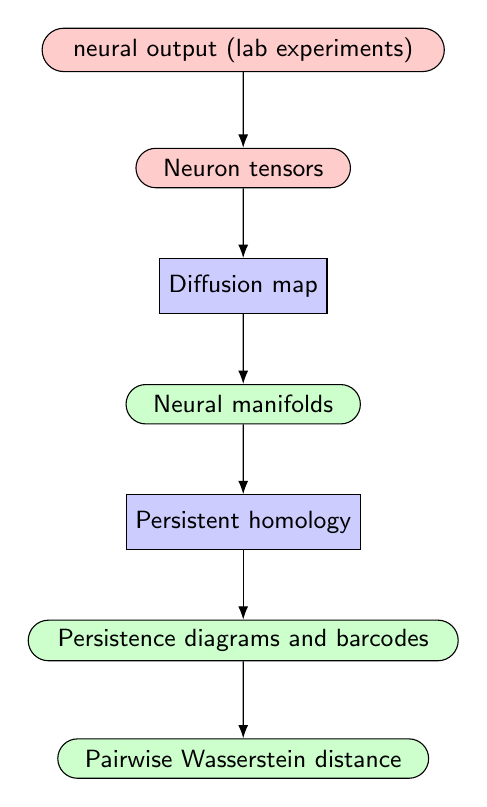
\begin{tikzpicture}[font={\sf \small}]
 \def\smbwd{2cm}
%   \node (BNN) at (-3,0.5) [draw, terminal, minimum width=\smbwd,  fill=yellow!20, minimum height=0.5cm] {Biological Neural Networks}; 
%   \node (ANN) at (2.7,0.5) [draw, terminal, minimum width=\smbwd,  fill=yellow!20, minimum height=0.5cm] {Artificial Neural Networks}; 
  %------------
  \node (experimental) at (0,-0.5) [draw, terminal, minimum width=\smbwd,  fill=red!20, minimum height=0.5cm]{neural output (lab experiments)};
%   \node (artificial) at (2.7,-1)[draw, terminal,minimum width=\smbwd,  fill=red!20, minimum height=0.5cm]{neuron output (simulations)};
  %------------
  \node (tensors) at (0,-2) [draw, terminal, minimum width=\smbwd,  fill=red!20, minimum height=0.5cm] {Neuron tensors}; 
  %------------
  
  \node (diffusion) at (0,-3.5) [draw, process, minimum width=\smbwd, fill=blue!20, minimum height=0.7cm] {Diffusion map};
  %------------
  
  \node (manifolds) at (0,-5) [draw, terminal, minimum width=\smbwd,  fill=green!20, minimum height=0.5cm] {Neural manifolds};
  
   \node (persistent) at (0,-6.5) [draw, process, minimum width=\smbwd, fill=blue!20, minimum height=0.7cm] {Persistent homology};
   
   \node (features) at (0,-8) [draw, terminal, minimum width=\smbwd,  fill=green!20, minimum height=0.5cm] {Persistence diagrams and barcodes};
   
   \node (wasserstein) at (0,-9.5) [draw, terminal, minimum width=\smbwd,  fill=green!20, minimum height=0.5cm] {Pairwise Wasserstein distance};
  
  %------------
  
%  \path [line](BNN) -- (experimental);
%  \path [line](ANN) -- (artificial);
 \path [line](tensors) -- (diffusion);
 \path [line](experimental) -- (tensors) ;
%  \path [line] (artificial) -- (tensors) ;
 \path [line](diffusion) -- (manifolds);
  \path [line](manifolds) -- (persistent);
   \path [line](persistent) -- (features);
  \path [line](features) -- (wasserstein); 
 \end{tikzpicture}
 
\section{Data Collection}

The neural spiking data (\cite{dyballa_manifold_2021}) were collected from lab experiments with the setup shown in the figure below. Six different types of flow stimuli developed in \cite{visual-flow} were flashed in front of the mouse. The electrodes recorded the neural output from the mouse's retina while it viewed each flow stimuli moving in eight directions respectively. The neural recordings were encoded in peristimulus (PSTH) diagrams, each of which showed the firing rate of one neuron over time for the eight directions respectively. In the PSTH diagram the brighter pixels indicate higher firing rates.
 \begin{figure}[H]
        \centering
            \includegraphics[width=0.55\textwidth]{figures/Slide5.jpg}
            \caption{Visualising neural data from lab experiments.}
    \end{figure}
    
\par The neural spiking data is of three dimensions: the first dimension represents the $698$ neurons; the second dimension represents the six different types of stimuli; the third dimension represents the vectorized PSTH diagrams, each of which has $8\times 33 = 264$ pixels. This gives us a $3$-way tensor:

\begin{defn}[Neural tensors]
    Suppose $\mathcal{S}$ is a set of flow stimuli $\mathcal{S} = \{s_1, s_2,\dots, s_K\}$, each moving over  $T$ time steps. The \underline{neural population response} of a set of $N$ neurons to some stimulus $s_i$ over time is $\mathcal{N} = \{\vec{n}_1, \vec{n}_2, \dots, \vec{n}_N\},$ where $\vec{n}_i \in \mathbb{R}^{T}$. 

    Each \underline{neural tensor} encodes the neural population response of $N$ neurons to $K$ flow stimuli over $T$ time steps and is thus a $3$-way $N$-by-$K$-by-$T$ tensor.
\end{defn}

With this neural spiking data set, we can create six point clouds, each corresponds to the neural population response towards one type of stimuli, which we denote as $X_1, X_2, \dots,X_6$. Each of the point cloud $X_i$ is thus represented by a matrix of dimension $698$-by-$264$, giving us a point cloud of $698$ points in $\RR^{264}$. 

\section{Step 1: Dimensionality Reduction}

The main motivation behind dimensionality reduction is that the intrinsic dimension of the data is usually much lower than the extrinsic dimension and the high-dimensionality is usually just an artifact of the representation. The representation of data has a potentially large degree of freedom, that is, the number of variables that are really necessary to describe the data is much smaller.

The Manifold Hypothesis states that real-world high-dimensional data lie on low-dimensional manifolds embedded within the high-dimensional space. (\cite{deepai_2019})

% main idea behind manifold learning:
In the context of neuroscience, neural spiking data is high-dimensional, but the neural connections constrain the possible patterns of population activity (\cite{okun_diverse_2015}, \cite{sadtler_neural_2014}, \cite{tsodyks_attractor_1999}) and that the possible patterns are confined to a low-dimensional manifold (\cite{stopfer_intensity_2003},  \cite{yu_gaussian-process_2009}) spanned by a few independent patterns that are called "neural modes." (\cite{gallego_neural_2017})

In terms of implementation, we used the pydiffmap package (\cite{eastman_pydiffmap_2017}). In our implementation, we reduced the dimensionaltity of each point cloud from the space of $\RR^{264}$ to $\RR^3$ using diffusion map. The resulting three-dimensional embedding of the original point clouds colored by the first three diffusion coordinates are shown below:
\begin{figure}[H]
\centering
\begin{subfigure}[b]{0.3\textwidth}
    \includegraphics[width=\textwidth]{figures/X1_embedding.png}
    \caption{Three-dimensional embedding of the original point cloud $X_1$.}
\end{subfigure}
\hfill
\begin{subfigure}[b]{0.3\textwidth}
    \includegraphics[width=\textwidth]{figures/X2_embedding.png}
    \caption{Three-dimensional embedding of the original point cloud $X_2$.}
\end{subfigure}
\hfill
\begin{subfigure}[b]{0.3\textwidth}
    \includegraphics[width=\textwidth]{figures/X3_embedding.png}
    \caption{Three-dimensional embedding of the original point cloud $X_3$.}
\end{subfigure}
\hfill
\begin{subfigure}[b]{0.3\textwidth}
    \includegraphics[width=\textwidth]{figures/X4_embedding.png}
    \caption{Three-dimensional embedding of the original point cloud $X_4$.}
\end{subfigure}
\hfill
\begin{subfigure}[b]{0.3\textwidth}
    \includegraphics[width=\textwidth]{figures/X5_embedding.png}
    \caption{Three-dimensional embedding of the original point cloud $X_5$.}
\end{subfigure}
\hfill
\begin{subfigure}[b]{0.3\textwidth}
    \includegraphics[width=\textwidth]{figures/X6_embedding.png}
    \caption{Three-dimensional embedding of the original point cloud $X_6$.}
\end{subfigure}
\end{figure}

\section{Step 2: Persistent Homology}

Having obtained the three-dimensional embeddings of the point clouds corresponding to six stimuli types, we applied persistent homology to extract the topological features from the six embeddings respectively. In this step, these topological features are represented by persistence barcodes and persistence diagrams.

Our implementation used the package ripser (\cite{ctralie2018ripser}) to obtain the respective persistence diagrams from the embeddings. Using the (birth, death)-intervals from each persistence diagram, we drew the equivalent persistence barcode representation. The complete code can be found in Appendix \ref{AppendixA}. The following figures show the results from applying persistent homology.
\begin{figure}[H]
\centering
\begin{subfigure}[b]{0.2\textwidth}
    \includegraphics[width=\textwidth]{figures/X1_embedding.png}
    \caption{Three-dimensional embedding of the original point cloud $X_1$.}
\end{subfigure}
\hfill
\begin{subfigure}[b]{0.75\textwidth}
    \includegraphics[width=\textwidth]{figures/X1_H0.png}
    \caption{Persistence diagrams.}
\end{subfigure}
\begin{subfigure}[b]{0.25\textwidth}
\includegraphics[width=\textwidth]{figures/white.png} 
\end{subfigure}
\begin{subfigure}[b]{0.24\textwidth}
    \includegraphics[width=\textwidth]{figures/X1_H0_barcode.png}
    \caption{}
\end{subfigure}
\begin{subfigure}[b]{0.24\textwidth}
    \includegraphics[width=\textwidth]{figures/X1_H1_barcode.png}
        \caption{Persistence barcodes.}
\end{subfigure}
\begin{subfigure}[b]{0.24\textwidth}
\includegraphics[width=\textwidth]{figures/X1_H2_barcode.png}
 \caption{}
\end{subfigure}
\caption{Results for applying persistent homology on the three-dimensional embedding of $X_1$.}
\end{figure}

\begin{figure}[H]
\centering
\begin{subfigure}[b]{0.2\textwidth}
    \includegraphics[width=\textwidth]{figures/X2_embedding.png}
    \caption{Three-dimensional embedding of the original point cloud $X_2$.}
\end{subfigure}
\hfill
\begin{subfigure}[b]{0.75\textwidth}
    \includegraphics[width=\textwidth]{figures/X2_H0.png}
    \caption{Persistence diagrams.}
\end{subfigure}
\begin{subfigure}[b]{0.25\textwidth}
\includegraphics[width=\textwidth]{figures/white.png} 
\end{subfigure}
\begin{subfigure}[b]{0.24\textwidth}
    \includegraphics[width=\textwidth]{figures/X2_H0_barcode.png}
    \caption{}
\end{subfigure}
\begin{subfigure}[b]{0.24\textwidth}
    \includegraphics[width=\textwidth]{figures/X2_H1_barcode.png}
        \caption{Persistence barcodes.}
\end{subfigure}
\begin{subfigure}[b]{0.24\textwidth}
\includegraphics[width=\textwidth]{figures/X2_H2_barcode.png}
 \caption{}
\end{subfigure}
\caption{Results for applying persistent homology on the three-dimensional embedding of $X_2$.}
\end{figure}

\begin{figure}[H]
\centering
\begin{subfigure}[b]{0.2\textwidth}
    \includegraphics[width=\textwidth]{figures/X3_embedding.png}
    \caption{Three-dimensional embedding of the original point cloud $X_3$.}
\end{subfigure}
\hfill
\begin{subfigure}[b]{0.75\textwidth}
    \includegraphics[width=\textwidth]{figures/X3_H0.png}
    \caption{Persistence diagrams.}
\end{subfigure}
\begin{subfigure}[b]{0.25\textwidth}
\includegraphics[width=\textwidth]{figures/white.png} 
\end{subfigure}
\begin{subfigure}[b]{0.24\textwidth}
    \includegraphics[width=\textwidth]{figures/X3_H0_barcode.png}
    \caption{}
\end{subfigure}
\begin{subfigure}[b]{0.24\textwidth}
    \includegraphics[width=\textwidth]{figures/X3_H1_barcode.png}
        \caption{Persistence barcodes.}
\end{subfigure}
\begin{subfigure}[b]{0.24\textwidth}
\includegraphics[width=\textwidth]{figures/X3_H2_barcode.png}
 \caption{}
\end{subfigure}
\caption{Results for applying persistent homology on the three-dimensional embedding of $X_3$.}
\end{figure}

\begin{figure}[H]
\centering
\begin{subfigure}[b]{0.2\textwidth}
    \includegraphics[width=\textwidth]{figures/X4_embedding.png}
    \caption{Three-dimensional embedding of the original point cloud $X_4$.}
\end{subfigure}
\hfill
\begin{subfigure}[b]{0.75\textwidth}
    \includegraphics[width=\textwidth]{figures/X4_H0.png}
    \caption{Persistence diagrams.}
\end{subfigure}
\begin{subfigure}[b]{0.25\textwidth}
\includegraphics[width=\textwidth]{figures/white.png} 
\end{subfigure}
\begin{subfigure}[b]{0.24\textwidth}
    \includegraphics[width=\textwidth]{figures/X4_H0_barcode.png}
    \caption{}
\end{subfigure}
\begin{subfigure}[b]{0.24\textwidth}
    \includegraphics[width=\textwidth]{figures/X4_H1_barcode.png}
        \caption{Persistence barcodes.}
\end{subfigure}
\begin{subfigure}[b]{0.24\textwidth}
\includegraphics[width=\textwidth]{figures/X4_H2_barcode.png}
 \caption{}
\end{subfigure}
\caption{Results for applying persistent homology on the three-dimensional embedding of $X_4$.}
\end{figure}

\begin{figure}[H]
\centering
\begin{subfigure}[b]{0.2\textwidth}
    \includegraphics[width=\textwidth]{figures/X5_embedding.png}
    \caption{Three-dimensional embedding of the original point cloud $X_5$.}
\end{subfigure}
\hfill
\begin{subfigure}[b]{0.75\textwidth}
    \includegraphics[width=\textwidth]{figures/X5_H0.png}
    \caption{Persistence diagrams.}
\end{subfigure}
\begin{subfigure}[b]{0.25\textwidth}
\includegraphics[width=\textwidth]{figures/white.png} 
\end{subfigure}
\begin{subfigure}[b]{0.24\textwidth}
    \includegraphics[width=\textwidth]{figures/X5_H0_barcode.png}
    \caption{}
\end{subfigure}
\begin{subfigure}[b]{0.24\textwidth}
    \includegraphics[width=\textwidth]{figures/X5_H1_barcode.png}
        \caption{Persistence barcodes.}
\end{subfigure}
\begin{subfigure}[b]{0.24\textwidth}
\includegraphics[width=\textwidth]{figures/X5_H2_barcode.png}
 \caption{}
\end{subfigure}
\caption{Results for applying persistent homology on the three-dimensional embedding of $X_5$.}
\end{figure}

\begin{figure}[H]
\centering
\begin{subfigure}[b]{0.2\textwidth}
    \includegraphics[width=\textwidth]{figures/X6_embedding.png}
    \caption{Three-dimensional embedding of the original point cloud $X_6$.}
\end{subfigure}
\hfill
\begin{subfigure}[b]{0.75\textwidth}
    \includegraphics[width=\textwidth]{figures/X6_H0.png}
    \caption{Persistence diagrams.}
\end{subfigure}
\begin{subfigure}[b]{0.25\textwidth}
\includegraphics[width=\textwidth]{figures/white.png} 
\end{subfigure}
\begin{subfigure}[b]{0.24\textwidth}
    \includegraphics[width=\textwidth]{figures/X6_H0_barcode.png}
    \caption{}
\end{subfigure}
\begin{subfigure}[b]{0.24\textwidth}
    \includegraphics[width=\textwidth]{figures/X6_H1_barcode.png}
        \caption{Persistence barcodes.}
\end{subfigure}
\begin{subfigure}[b]{0.24\textwidth}
\includegraphics[width=\textwidth]{figures/X6_H2_barcode.png}
 \caption{}
\end{subfigure}
\caption{Results for applying persistent homology on the three-dimensional embedding of $X_6$.}
\end{figure}

\section{Step 3: Pairwise Wasserstein distance}
In the last step, we used the gudhi package (\cite{gudhi:urm}) to compute the pairwise Wasserstein distance between the persistence diagrams. The method used is based on (\cite{kerber_geometry_2016}). 

We first computed the first pairwise distances between the persistence diagrams for each of the six point clouds. 

\begin{table}[!htbp]
        \centering
        \small
        \setlength\tabcolsep{5pt}
        \begin{tabular}{|c|c|c|c|c|c|c|}
\hline
 $H_0$& $X_1$ & $X_2$ & $X_3$ & $X_4$ & $X_5$ & $X_6$\\
 \hline
$X_1$ &
0.0&
2.77&
3.05&
3.95&
3.08&
3.42
\\
\hline
$X_2$ &
2.77&
0.0&
0.43&
1.35&
1.0&
0.84
\\
\hline
$X_3$ &
3.05&
0.43&
0.0&
1.03&
0.94&
0.66
\\
\hline
$X_4$ &
3.95&
1.35&
1.03&
0.0&
1.11&
0.72
\\
\hline
$X_5$ &
3.08&
1.0&
0.94&
1.11&
0.0&
0.51
\\
\hline
$X_6$ &
3.42&
0.84&
0.66&
0.72&
0.51&
0.0
\\
\hline
\end{tabular}
\caption{Pairwise Wasserstein distance between persistent diagrams for homology group $H_0$.}
\label{tab:Wass_H0}
\end{table}

\begin{table}[!htbp]
        \centering
        \small
        \setlength\tabcolsep{5pt}
        \begin{tabular}{|c|c|c|c|c|c|c|}
\hline
 $H_1$& $X_1$ & $X_2$ & $X_3$ & $X_4$ & $X_5$ & $X_6$ \\ \hline
$X_1$ &
0.0&
0.46&
0.5&
0.64&
0.64&
0.55

\\\hline
$X_2$ &
0.46&
0.0&
0.17&
0.29&
0.36&
0.3
\\\hline
$X_3$ &
0.5&
0.17&
0.0&
0.25&
0.33&
0.3
\\\hline 
$X_4$ &
0.64&
0.29&
0.25&
0.0&
0.27&
0.29
\\\hline 
$X_5$ &
0.64&
0.36&
0.33&
0.27&
0.0&
0.26

\\\hline
$X_6$ &
0.55&
0.3&
0.3&
0.29&
0.26&
0.0\\
\hline
\end{tabular}
\caption{Pairwise Wasserstein distance between persistent diagrams for homology group $H_1$.}
\label{tab:Wass_H1}
\end{table}

\begin{table}[!htbp]
        \centering
        \small
        \setlength\tabcolsep{5pt}
        \begin{tabular}{|c|c|c|c|c|c|c|}
\hline
 $H_2$& $X_1$ & $X_2$ & $X_3$ & $X_4$ & $X_5$ & $X_6$ \\ \hline
$X_1$ &
0.0&
0.06&
0.06&
0.06&
0.06&
0.06
\\
\hline
$X_2$ &
0.06&
0.0&
0.01&
0.0&
0.01&
0.0
\\
\hline
$X_3$ &
0.06&
0.01&
0.0&
0.0&
0.01&
0.0
\\
\hline
$X_4$ &
0.06&
0.0&
0.0&
0.0&
0.0&
0.0
\\
\hline
$X_5$ &
0.06&
0.01&
0.01&
0.0&
0.0&
0.0
\\
\hline
$X_6$ &
0.06&
0.0&
0.0&
0.0&
0.0&
0.0
\\
\hline
\end{tabular}
\caption{Pairwise Wasserstein distance between persistent diagrams for homology group $H_2$.}
\label{tab:Wass_H2}
\end{table}

Building upon the same method, we further compared the six point clouds with known three-dimensional shapes ($2$-sphere and torus) based on the Wasserstein distance.

First, we extracted the topological features of the $2$-sphere and three-dimensional torus, as we did for the point clouds in Step 2. 
\begin{figure}[H]
\centering
\begin{subfigure}[b]{0.2\textwidth}
    \includegraphics[width=\textwidth]{figures/dsphere.png}
    \caption{Scatter plot for $2$-sphere.}
\end{subfigure}
\hfill
\begin{subfigure}[b]{0.75\textwidth}
    \includegraphics[width=\textwidth]{figures/dsphere_Hk.png}
    \caption{Persistence diagrams.}
\end{subfigure}
\begin{subfigure}[b]{0.25\textwidth}
\includegraphics[width=\textwidth]{figures/white.png} 
\end{subfigure}
\begin{subfigure}[b]{0.24\textwidth}
    \includegraphics[width=\textwidth]{figures/dsphere_H0_barcode.png}
    \caption{}
\end{subfigure}
\begin{subfigure}[b]{0.24\textwidth}
    \includegraphics[width=\textwidth]{figures/dsphere_H1_barcode.png}
        \caption{Persistence barcodes.}
\end{subfigure}
\begin{subfigure}[b]{0.24\textwidth}
\includegraphics[width=\textwidth]{figures/dsphere_H2_barcode.png}
 \caption{}
\end{subfigure}
\caption{Results for applying persistent homology on the $2$-sphere.}
\end{figure}

\begin{figure}[H]
\centering
\begin{subfigure}[b]{0.2\textwidth}
    \includegraphics[width=\textwidth]{figures/torus.png}
    \caption{Scatter plot for the three-dimensional torus.}
\end{subfigure}
\hfill
\begin{subfigure}[b]{0.75\textwidth}
    \includegraphics[width=\textwidth]{figures/torus_Hk.png}
    \caption{Persistence diagrams.}
\end{subfigure}
\begin{subfigure}[b]{0.25\textwidth}
\includegraphics[width=\textwidth]{figures/white.png} 
\end{subfigure}
\begin{subfigure}[b]{0.24\textwidth}
    \includegraphics[width=\textwidth]{figures/torus_H0_barcode.png}
    \caption{}
\end{subfigure}
\begin{subfigure}[b]{0.24\textwidth}
    \includegraphics[width=\textwidth]{figures/torus_H1_barcode.png}
        \caption{Persistence barcodes.}
\end{subfigure}
\begin{subfigure}[b]{0.24\textwidth}
\includegraphics[width=\textwidth]{figures/torus_H2_barcode.png}
 \caption{}
\end{subfigure}
\caption{Results for applying persistent homology on the three-dimensional torus.}
\end{figure}

Then, we computed the Wasserstein distance between the six point clouds and the known shapes:

\begin{table}[!htbp]
        \centering
        \small
        \setlength\tabcolsep{5pt}
        \begin{tabular}{|c|c|c|c|c|c|c|}
\hline
  $H_0$& $X_1$ & $X_2$ & $X_3$ & $X_4$ & $X_5$ & $X_6$ \\ \hline
$2$-sphere & 2.48 & 4.46&  4.64 & 5.18 & 4.53 & 4.83\\\hline
torus & 3.63 &  1.46 & 1.31 & 0.73 & 1.38 & 1.06 \\ \hline
\end{tabular}
\caption{Wasserstein distance between persistent diagrams of the point clouds and $2$-sphere and torus (homology group $H_0$).}
\label{tab:sphere-H0}
\end{table}


\begin{table}[!htbp]
        \centering
        \small
        \setlength\tabcolsep{5pt}
        \begin{tabular}{|c|c|c|c|c|c|c|}
\hline
$H_1$& $X_1$ & $X_2$ & $X_3$ & $X_4$ & $X_5$ & $X_6$ \\ \hline
$2$-sphere & 0.62 &   0.77 & 0.80 & 0.87 & 0.85 & 0.76\\\hline
torus & 0.74 & 0.49 & 0.44 & 0.34 & 0.45 & 0.47\\ \hline
\end{tabular}
\caption{Wasserstein distance between persistent diagrams of the point clouds and $2$-sphere and torus (homology group $H_1$).}
\label{tab:sphere-H1}
\end{table}

\begin{table}[!htbp]
        \centering
        \small
        \setlength\tabcolsep{5pt}
        \begin{tabular}{|c|c|c|c|c|c|c|}
\hline
$H_2$ & $X_1$ & $X_2$ & $X_3$ & $X_4$ & $X_5$ & $X_6$ \\ \hline
$2$-sphere & 0.11 &   0.12 & 0.12 & 0.12 & 0.13 & 0.12\\\hline
torus & 0.057 & 0.017 & 0.018  & 0.016 & 0.018 & 0.016 \\ \hline
\end{tabular}
\caption{Wasserstein distance between persistent diagrams of the point clouds and $2$-sphere and torus (homology group $H_2$).}
\label{tab:sphere-H2}
\end{table}

\section{Analysis of results}
Based on the results from the above tables of Wasserstein distances, our observations and inferences are as follows.

\begin{enumerate}
    \item The topological structure for $X_1$ is distinct from the rest. 
    
    Based on the pairwise Wasserstein distances in Tables \ref{tab:Wass_H0} and \ref{tab:Wass_H1}, $X_1$ is notably different from the rest of the point clouds in terms of topological structure. In the context of our application, this implies that the neural population response evoked by stimulus type 1 is significantly different from the other stimulus types. This observation leads us to hypothesize that there is some neuroscientific reason behind this distinction in the topological structure of neural population response. It might be interesting to conduct further lab experiments to investigate what special properties this stimulus has and why it causes such different  neural population response. 
    
    \item Wasserstein distances between persistence diagrams are nearly negligible for $H_2$.
    
    Based on Table \ref{tab:Wass_H2}, pairwise Wasserstein distances between persistence diagrams for $H_2$ are small enough to be nearly negligible. This implies that the intrinsic dimensionality of this neural data might be even lower than three-dimensional since there is no significant differences in homology groups $H_2$ for the point clouds.
    
    \item Shape comparison with $2$-sphere and torus.
    
    Based on Tables \ref{tab:sphere-H0} and \ref{tab:sphere-H1}, the Wasserstein distances between the point clouds and the $2$-sphere are smaller than the Wasserstein distances between the point clouds and the torus for all $X_i$ except for $X_1$. We can thus infer that except for $X_1$, all other point clouds are more similar to the shape of a torus than the $2$-sphere. This implies that the topological structure of the neural population response evoked by stimuli type 1 is more similar to a sphere while the neural population response evoked by the rest of the stimuli types used in the experiments are more similar to a torus. 
    
    It would be interesting to compare this result with the hypothesis in (\cite{ben-yishai_theory_1995}, \cite{Blumenfeld_2006}, \cite{goldberg_randomized_2004},    \cite{singh_top_v1_2008}):
    If we are given an oriented stimulus, and if the orientation is a circular variable, then the hypothesis is that the neural population response evoked by such stimulus must have a topological structure equivalent to that of a circle. However, to fully test this hypothesis, further experiments with different types of stimuli need to be conducted.
\end{enumerate}

\section{Conclusion}
In this chapter, we demonstrated our proposed approach to compare the point clouds that represent the neural population response to different stimuli. Our proposed approach is contingent on the topological structures of the point clouds.  

One significant limitation in this specific application is that lab data usually involve a lot of sampling errors such as missing data and inconsistent densities, causing noise to the true underlying geometry of the neural population response. Persistent homology works well on synthetic data, but might not work when the sampling errors are too significant.

The advantages of topological approach is that we can provide a succinct and useful summary of the global geometric structure of the neural spiking data, thus obtaining a useful account of how similarly the neurons collectively respond to visual stimuli. This is especially important in applications where the notion of connectedness and clusters are salient. As an emerging field, TDA will certainly see more applications in solving problems that involve understanding the geometric and topological structure of high-dimensional data.

\printbibliography[heading=bibintoc]


\appendix 
\input{appendix/appendixA}

\end{document}
